\documentclass{article}

\usepackage{float}
\usepackage{xcolor}
\usepackage{parskip}
\usepackage{eulervm}
\usepackage{graphicx}
\usepackage{setspace}
\usepackage{geometry}
\usepackage{mathpazo}
\usepackage{microtype}
\usepackage[T1]{fontenc}
\usepackage[utf8]{inputenc}
\usepackage{amsfonts, amsmath, amssymb}

\setstretch{1.50}
\geometry{paper=letterpaper, layout=letterpaper, margin=1in}

\begin{document}

\begin{titlepage}
    \begin{center}
        \vspace*{2cm}
        {\Huge \textbf{ ME 4638: Computational Mechanics Lab}} \\
        \vspace{1cm}
        \Large{\textbf{Assignment II}} \\

        \vfill

        \textit{\large Submitted by:} \\
        \vspace{0.3cm}
        \textbf{Abdullah al Azmi} \\
        \textbf{ID: 220011230} \\

        \vfill

        \textit{\large Submitted to:} \\
        \vspace{0.3cm}
        \textbf{\Large Sefat Mahmud Siddique (Junior Lecturer)} \\
        \textbf{Department of Mechanical and Production Engineering} \\

        \vfill

        \textbf{Date of Submission: \today}
        \vspace*{1cm}
    \end{center}
\end{titlepage}

\newpage

\setcounter{section}{3}

\section{Prediction}

\begin{itemize}
    \item [a.] A fixed constraint is required to prevent rigid body motion. Without it, the static solver cannot reach equilibrium because the structure would float away under the applied loads, leading to a singular matrix error.
    \item [b.] Hexahedral elements are difficult to map onto cylindrical geometries like the post. This often leads to highly distorted elements or mesh failure.
    \item [c.] To solve the problem, one should use tetrahedral elements or multizone meshing instead, which can better conform to complex geometries.
    \item [d.] The choice of 5 inches for both components is a balance between computational cost and accuracy. It ensures there are enough elements to capture the stress distribution without making the problem too large to solve efficiently.
    \item [e.] The constraint must be placed at the base of the steel post (Fixed Support). This replicates the real-world scenario where the post is anchored to the ground, providing a realistic boundary condition for the analysis.
    \item [f \& g.] The expected deformation for weight of the sign and the spatially varying wind pressure is given below:
          \begin{figure} [H]
              \centering
              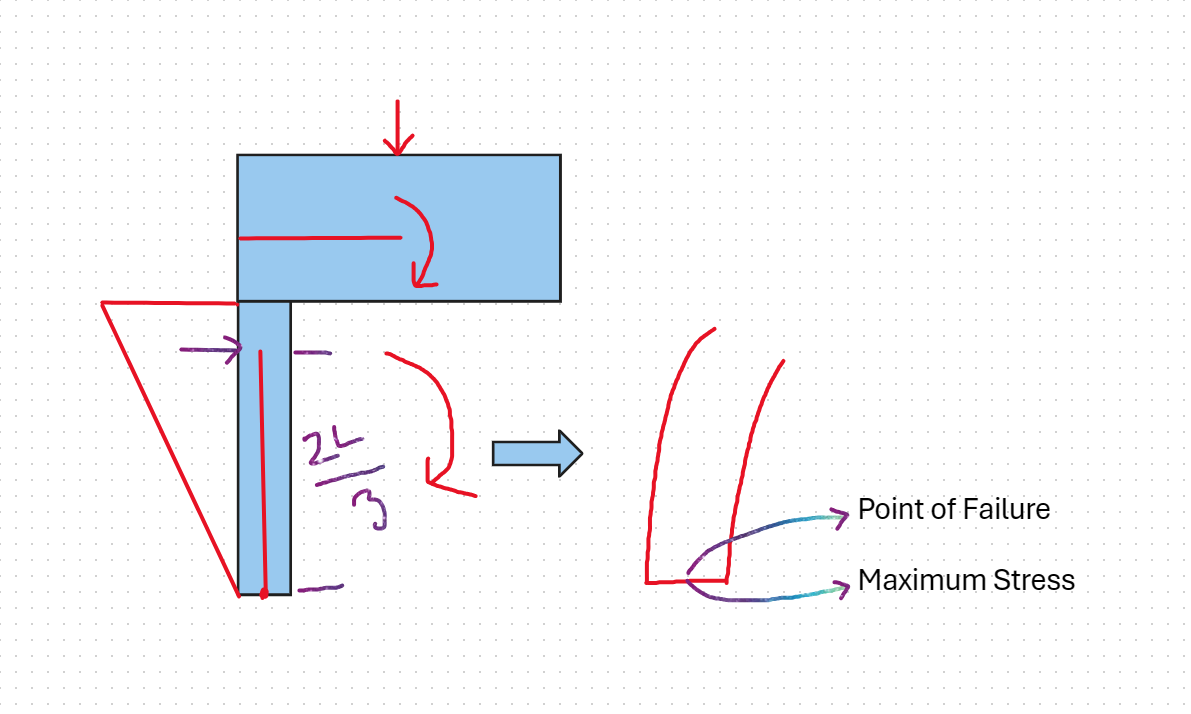
\includegraphics[width=0.8\textwidth]{images/rough_sketch.png}
              \caption{Rough sketch of the expected structure deformation and location of max. stress and point of failure.}
          \end{figure}
    \item[h.] The maximum stress is expected to occur at the base of the post where it is fixed, due to the bending moment caused by the wind load and the weight of the sign. The point of failure is likely to be at this location as well, as it will experience the highest stress concentration.
\end{itemize}

\section{Analysis Results}

\begin{itemize}
    \item [a.] The screenshots of the required solution fields are shown below:
          \begin{itemize}
              \item[] \begin{figure} [H]
                        \centering
                        
\includegraphics[width=0.8\textwidth]{images/total_deformation.png}
                        \caption{Total deformation of the structure under the applied loads.}
                    \end{figure}
              \item[] \begin{figure} [H]
                        \centering
                        
\includegraphics[width=0.8\textwidth]{images/normal_stress_at_x_direction.png}
                        \caption{Normal stress distribution at X-direction in the structure.}
                    \end{figure}
              \item[] \begin{figure} [H]
                        \centering
                        
\includegraphics[width=\textwidth]{images/normal_stress_at_y_direction.png}
                        \caption{Normal stress distribution at Y-direction in the structure.}
                    \end{figure}
              \item[] \begin{figure} [H]
                        \centering
                        
\includegraphics[width=\textwidth]{images/normal_stress_at_z_direction.png}
                        \caption{Normal stress distribution at Z-direction in the structure.}
                    \end{figure}
              \item[] \begin{figure} [H]
                        \centering
                        
\includegraphics[width=\textwidth]{images/max_shear_stress.png}
                        \caption{Maximum shear stress distribution in the structure.}
                    \end{figure}
              \item[] \begin{figure} [H]
                        \centering
                        
\includegraphics[width=\textwidth]{images/equivalent_stress.png}
                        \caption{Equivalent stress distribution in the structure.}
                    \end{figure}
              \item[] \begin{figure} [H]
                        \centering
                        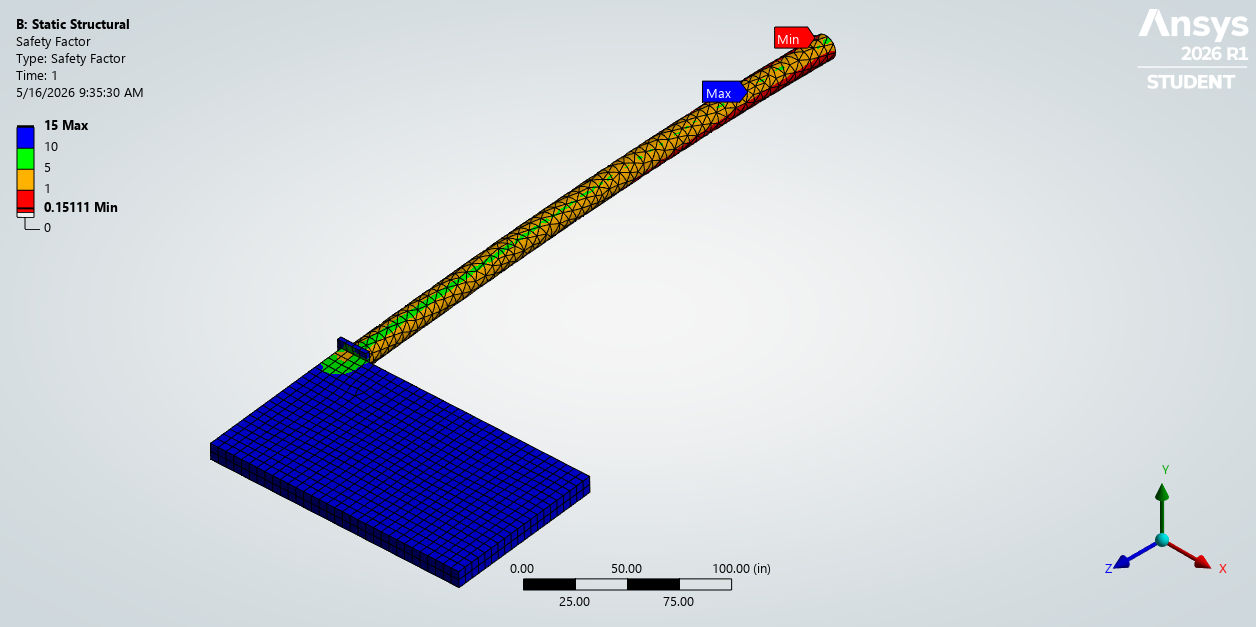
\includegraphics[width=\textwidth]{images/max_shear_stress_fos.png}
                        \caption{Factor of safety against shear failure.}
                    \end{figure}
              \item[] \begin{figure} [H]
                        \centering
                        
\includegraphics[width=\textwidth]{images/max_tensile_stress_fos.png}
                        \caption{Factor of safety against tensile stress failure.}
                    \end{figure}
          \end{itemize}
    \item [b.] The equivalent stress and normal stress at Z-direction shows the maximum stress value. This is because the vertical loads and bending moments create significant longitudinal stress in the post.
    \item [c.] Equivalent shear stress is a useful metric for ductile materials like (steel and aluminum) as it combines all stress components into a single value to compare against the tensile yield strength. However, since separate shear and normal strength are provided, a maximum shear stress theory might be more conservative and specific for this analysis.
    \item [d.] A 3 times mesh refinement has been added at the region of maximum stress.
    \item [e.] The stress values specially the normal stress at X-direction has changed significantly from max 7810 psi to max 10366 psi. Also, the other stress values have changed as well.
    \item [f.] The maximum normal stress values at Y-direction is 22744 psi, which is slightly lower than the normal stress yield strength of 2500 psi. So, I think the signpost will not fail under the given loading conditions. However, it is important to consider factors such as fatigue and potential stress concentrations that could lead to failure over time.
\end{itemize}

\section{Post Design}

\section{Different Loading Scenarios}

\end{document}